\documentclass[11pt]{article}
\usepackage[T1]{fontenc}
\usepackage[utf8]{inputenc}
\usepackage[english]{babel}
\usepackage{lmodern,microtype,amsmath,amssymb,booktabs,graphicx,geometry,hyperref}
\geometry{a4paper,margin=2.4cm}
\hypersetup{hidelinks,pdftitle={Supplementary Computational Material: Manuscript v0.41},pdfauthor={Rodrigo Castro Marin}}
\renewcommand{\thetable}{S\arabic{table}}
\renewcommand{\thefigure}{S\arabic{figure}}
\title{Supplementary Computational Material\\\large Predictor-memory frozen-Jacobian methods, manuscript v0.41}
\author{Rodrigo Castro Mar\'in}
\date{}
\begin{document}\maketitle
This document is the English counterpart of the computational supplement accompanying manuscript v0.41. It preserves the numerical breakdowns removed from the main article during editorial compression; no essential proof has been moved here. All times below are archived measurements, not fresh measurements from the repository build. The manuscript itself remains a separate document.

\section{Detailed external-comparator timings}
Tables~\ref{tab:p5} and~\ref{tab:p7} retain the results at $\mathrm{TOL}=10^{-12}$. The main article summarizes all nine configurations per field. Full-precision CSV files, including the other tolerances, are supplied in \texttt{data/reference/p5\_m6\_results.csv} and \texttt{p7\_m8\_results.csv}.
The relative quantities are $\Delta t=100(t_A/t_B-1)$ and $\Delta W=100(W_A/W_B-1)$ for $\kappa=1$; negative values favor method $A$. Parentheses contain the IQR, in the same units as the median. The time separation rule is $|\widetilde t_A-\widetilde t_B|>2(\mathrm{IQR}_A+\mathrm{IQR}_B)$; it is descriptive, not a formal statistical test.
\begin{table}[htbp]\centering\small
\caption{Comparison $P_5/M6$ at $\mathrm{TOL}=10^{-12}$. Times and IQRs are in milliseconds.}\label{tab:p5}
\setlength{\tabcolsep}{4pt}
\begin{tabular}{cccrrrr}\toprule
Field & $\delta$ & Cycles & $P_5$ time (IQR) & $M6$ time (IQR) & $\Delta t$ [\%] & $\Delta W$ [\%]\\\midrule
$H_1$ & 0.10 & 1/1 & 0.1258 (0.0064) & 0.1252 (0.0075) & +0.48 & +6.78\\
$H_1$ & 0.30 & 2/2 & 0.2478 (0.0107) & 0.2428 (0.0175) & +2.06 & +8.89\\
$H_1$ & 0.60 & 2/2 & 0.2495 (0.0151) & 0.2423 (0.0124) & +2.97 & +8.89\\
$H_2$ & 0.10 & 1/1 & 0.1752 (0.0104) & 0.1747 (0.0124) & +0.29 & +5.91\\
$H_2$ & 0.30 & 1/1 & 0.1730 (0.0136) & 0.1731 (0.0141) & -0.06 & +5.91\\
$H_2$ & 0.60 & 2/2 & 0.3514 (0.0263) & 0.3362 (0.0186) & +4.52 & +7.37\\
$H_3$ & 0.10 & 1/1 & 0.2442 (0.0389) & 0.2506 (0.0310) & -2.55 & +3.97\\
$H_3$ & 0.30 & 1/1 & 0.2411 (0.0127) & 0.2499 (0.0207) & -3.52 & +3.97\\
$H_3$ & 0.60 & 2/2 & 0.4778 (0.0132) & 0.4909 (0.0275) & -2.67 & +4.98\\
$H_4$ & 0.10 & 1/1 & 0.5495 (0.0301) & 0.5704 (0.0699) & -3.66 & +3.08\\
$H_4$ & 0.30 & 1/1 & 0.5505 (0.0356) & 0.5772 (0.0552) & -4.63 & +3.08\\
$H_4$ & 0.60 & 2/2 & 1.1382 (0.1175) & 1.1402 (0.1064) & -0.18 & +3.84\\
$H_5$ & 0.10 & 1/1 & 1.0378 (0.0843) & 1.0821 (0.1272) & -4.09 & +2.44\\
$H_5$ & 0.30 & 1/1 & 1.0760 (0.0742) & 1.1164 (0.0804) & -3.62 & +2.44\\
$H_5$ & 0.60 & 2/2 & 2.0588 (0.1305) & 2.1217 (0.2128) & -2.96 & +3.05\\
\bottomrule
\end{tabular}
\end{table}
\clearpage
\begin{table}[htbp]\centering\small
\caption{Comparison $P_7/M8$ at $\mathrm{TOL}=10^{-12}$. Times and IQRs are in milliseconds.}\label{tab:p7}
\setlength{\tabcolsep}{4pt}
\begin{tabular}{cccrrrr}\toprule
Field & $\delta$ & Cycles & $P_7$ time (IQR) & $M8$ time (IQR) & $\Delta t$ [\%] & $\Delta W$ [\%]\\\midrule
$H_1$ & 0.10 & 1/1 & 0.1537 (0.0084) & 0.1202 (0.0050) & +27.87 & +15.71\\
$H_1$ & 0.30 & 1/1 & 0.1558 (0.0102) & 0.1220 (0.0108) & +27.70 & +15.71\\
$H_1$ & 0.60 & 2/2 & 0.3057 (0.0103) & 0.2274 (0.0088) & +34.43 & +17.94\\
$H_2$ & 0.10 & 1/1 & 0.2047 (0.0096) & 0.1774 (0.0155) & +15.39 & -5.07\\
$H_2$ & 0.30 & 1/1 & 0.2128 (0.0139) & 0.1808 (0.0169) & +17.70 & -5.07\\
$H_2$ & 0.60 & 1/1 & 0.2103 (0.0115) & 0.1801 (0.0106) & +16.77 & -5.07\\
$H_3$ & 0.10 & 1/1 & 0.2850 (0.0176) & 0.2844 (0.0148) & +0.21 & -23.53\\
$H_3$ & 0.30 & 1/1 & 0.2873 (0.0162) & 0.2856 (0.0116) & +0.60 & -23.53\\
$H_3$ & 0.60 & 1/1 & 0.2869 (0.0123) & 0.2881 (0.0168) & -0.42 & -23.53\\
$H_4$ & 0.10 & 1/1 & 0.5839 (0.0392) & 0.7361 (0.0495) & -20.68 & -30.59\\
$H_4$ & 0.30 & 1/1 & 0.6107 (0.0744) & 0.7729 (0.0663) & -20.99 & -30.59\\
$H_4$ & 0.60 & 1/1 & 0.5947 (0.0471) & 0.7348 (0.1047) & -19.07 & -30.59\\
$H_5$ & 0.10 & 1/1 & 1.1568 (0.0984) & 1.7986 (0.1976) & -35.68 & -34.90\\
$H_5$ & 0.30 & 1/1 & 1.0842 (0.0818) & 1.6504 (0.1198) & -34.31 & -34.90\\
$H_5$ & 0.60 & 1/1 & 1.0758 (0.0352) & 1.6450 (0.1357) & -34.60 & -34.90\\
\bottomrule
\end{tabular}
\end{table}
\section{Full sensitivity of the optimal members}
Table~\ref{tab:optima} retains all six control points. The main article displays two representative endpoints. Stability throughout $[1,4.5]$ follows from affine normalized-cost differences and the unimodality argument, not from this finite list alone.
\begin{table}[htbp]\centering\scriptsize
\caption{Stationary family optima and 0.5\% near-optimal bands.}\label{tab:optima}
\setlength{\tabcolsep}{4pt}
\begin{tabular}{ccrrrrrrl}\toprule
Field & $\kappa$ & $N_P^*$ & $m_S^*$ & $10^6\eta_P^*$ & $10^6\eta_S^*$ & Advantage [\%] & & P/S bands\\\midrule
$H_1$ & 1 & 3 & 3 & 172.461715 & 165.035043 & 4.50 & & $\{3\}/\{3\}$\\
$H_1$ & 1.2 & 3 & 3 & 171.409882 & 164.058504 & 4.48 & & $\{3\}/\{3\}$\\
$H_1$ & 1.298 & 3 & 3 & 170.899153 & 163.584207 & 4.47 & & $\{3\}/\{3\}$\\
$H_1$ & 1.7 & 3 & 3 & 168.835587 & 161.666981 & 4.43 & & $\{3\}/\{3\}$\\
$H_1$ & 3.23511 & 3 & 3 & 161.393776 & 154.741466 & 4.30 & & $\{3\}/\{3\}$\\
$H_1$ & 4.45444 & 3 & 3 & 155.934456 & 149.649474 & 4.20 & & $\{3\}/\{3\}$\\
$H_5$ & 1 & 9 & 10 & 0.555516 & 0.543469 & 2.22 & & $\{8,9,10,11\}/\{9,10,11\}$\\
$H_5$ & 1.2 & 9 & 10 & 0.554944 & 0.542925 & 2.21 & & $\{8,9,10,11\}/\{9,10,11\}$\\
$H_5$ & 1.298 & 9 & 10 & 0.554664 & 0.542659 & 2.21 & & $\{8,9,10,11\}/\{9,10,11\}$\\
$H_5$ & 1.7 & 9 & 10 & 0.553518 & 0.541570 & 2.21 & & $\{8,9,10,11\}/\{9,10,11\}$\\
$H_5$ & 3.23511 & 9 & 10 & 0.549186 & 0.537452 & 2.18 & & $\{8,9,10,11\}/\{9,10,11,12\}$\\
$H_5$ & 4.45444 & 9 & 10 & 0.545794 & 0.534226 & 2.17 & & $\{8,9,10,11\}/\{9,10,11,12\}$\\
\bottomrule\end{tabular}\end{table}
\clearpage
\section{Secondary graphical representations}
Figures~\ref{fig:external} and~\ref{fig:fusion} preserve the secondary comparisons. All labels are in English; the underlying measurements are unchanged. A configuration range is not an IQR or confidence interval. No interpolation establishes a universal time crossover or monotonicity.
\begin{figure}[htbp]\centering
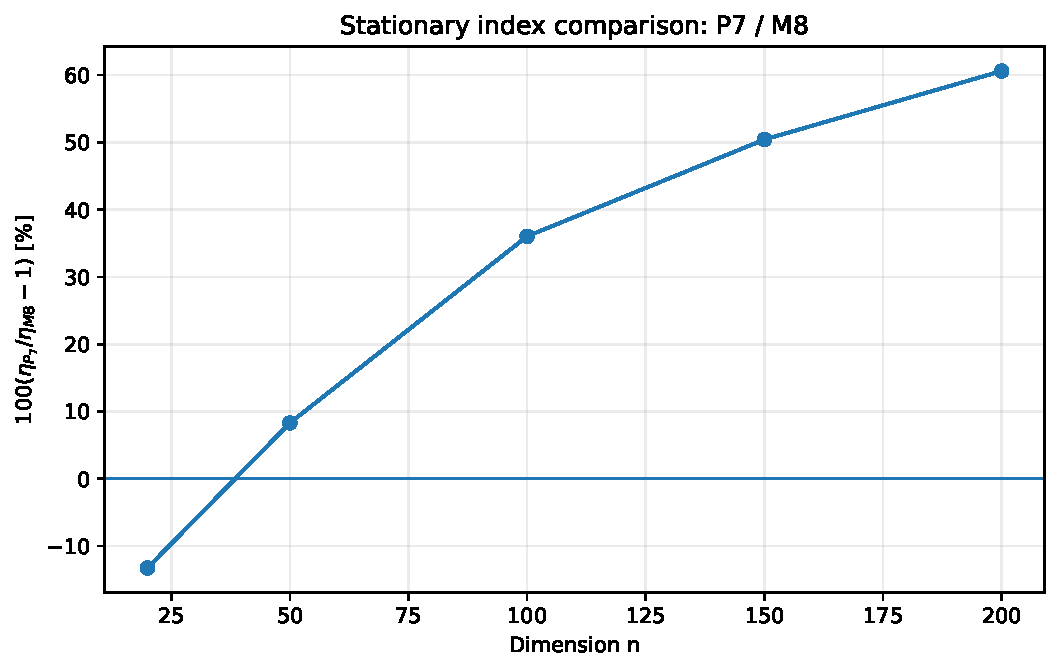
\includegraphics[width=.49\textwidth]{supp_figS1_index.pdf}\hfill
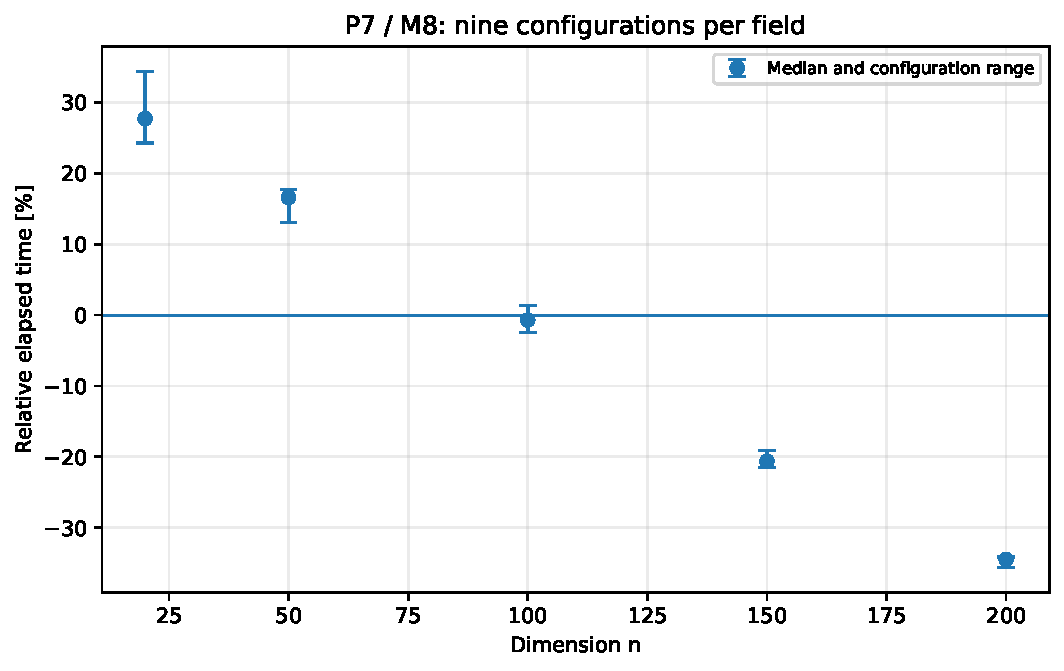
\includegraphics[width=.49\textwidth]{supp_figS1_time.pdf}
\caption{$P_7/M8$: stationary index advantage (left) and median with range of relative elapsed time over nine configurations per field (right). Positive index differences and negative time differences favor $P_7$. Time-separation decisions are made separately for each configuration.}\label{fig:external}
\end{figure}
\begin{figure}[htbp]\centering
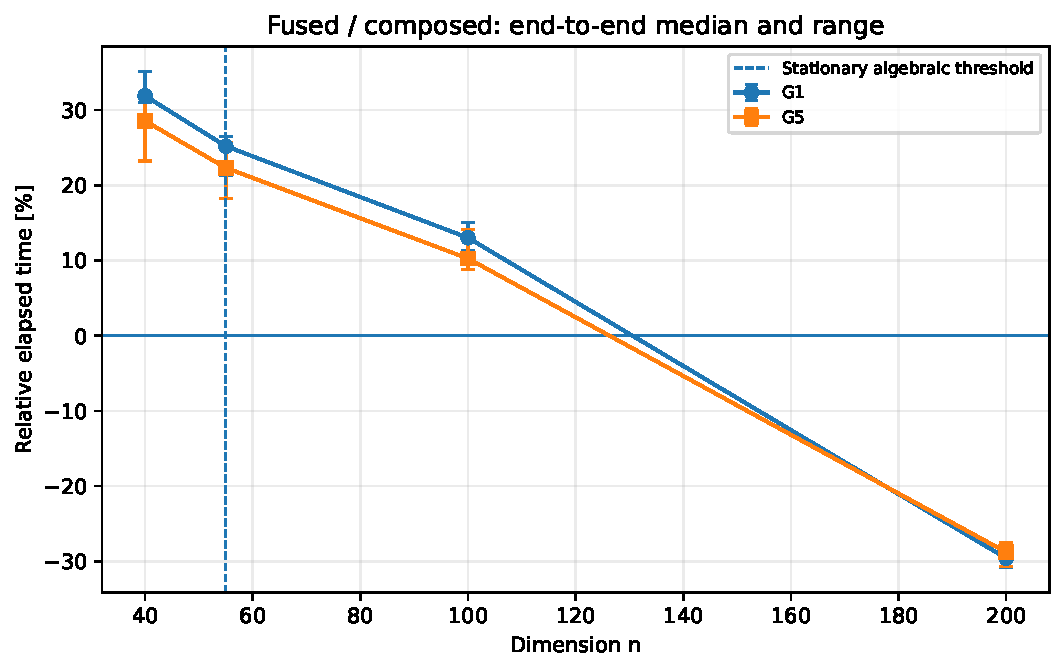
\includegraphics[width=.79\textwidth]{supp_figS2_fusion.pdf}
\caption{End-to-end comparison of $\widehat P_2$ with $P_2\circ P_2$: median and range of relative elapsed time. The line $n=55$ is the stationary algebraic threshold, not an estimated temporal crossover. Negative values favor fusion.}\label{fig:fusion}
\end{figure}
\paragraph{Provenance note.} The archived fusion work columns for $G_5$ retain a historical evaluation-cost convention described in \texttt{docs/KNOWN\_ISSUES.md}. The elapsed-time values in Figure~\ref{fig:fusion} are unaffected. The repository preserves those inputs and provides the separately recomputed canonical costs; no measurement is silently replaced.
\end{document}
